% Ch3 Algorithm
\chapter{路徑規劃}
\label{c:algorithm}

本論文利用目標點位置與車輛位置之間的相對關係,以及車輛本身相對於地面的方位角,
計算出目標點相對於車輛的角度$\Theta_t$與最短距離$\sigma_t$。
由於位置單位為經緯度,\ref{sec:target}節介紹了由經緯度計算$\Theta_t$與$\sigma_t$
之方法。而利用$\Theta_t$、$\sigma_t$與光學雷達所得到的環境資訊,
本論文基於VFH+~\cite{Ulrich:1998:VFHPlus}開發出一避障演算法計算出前進方向,
以避開障礙物,\ref{sec:vfhplus}節介紹其架構。

\section{目標方向計算}
\label{sec:target}

\subsection{地理座標系統}
地理座標系統(Geographic Coordinate System)是用來表示地球上某個位置的座標系統,
這些座標系統可分為兩類:ECI(Earth Centered Inertial)與ECEF(Earth Centered Earth Fixed),
兩者之原點皆位於地球質心,但前者之座標系統不隨地球自轉而轉動,
座標軸永遠指向固定的方向(相對於星星);而後者之座標軸固定於地球上。
前者一般使用於天文學,像是找尋衛星的軌道等;
後者則多用來表示物體於地球上的位置,如GPS即使用ECEF系統。
簡單的ECEF座標系統可以用三維卡式座標系來表示,其原點位於地球的質心,
XY平面與地球的赤道平面重合,X軸指向經度$0\,^{\circ}$,
Y軸則是指向東經$90\,^{\circ}$,如圖~\ref{f:ecef}所示。
\begin{figure}[h!]
	\centering
	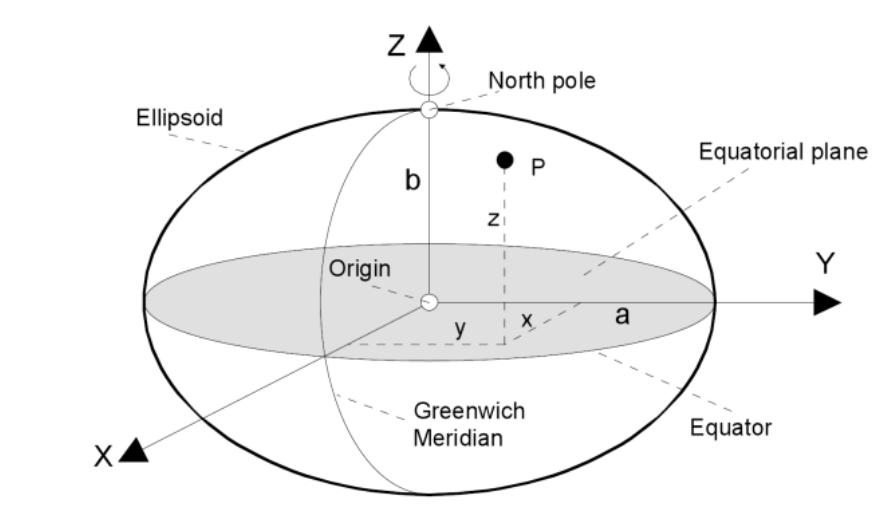
\includegraphics[width=12cm]{figures/ECEF}
	\caption{ECEF座標系統}
	\caption*{來源:MTi-G Manual}
	\label{f:ecef}
\end{figure}

雖然能夠使用各種座標系統來表示位置,但一般最常使用的是ECEF橢球座標系(Ellipsoidal Coordinates),
使用緯度(Latitude)$\phi$、經度(Longitude)$\lambda$與高度(Altitude)$h$來表示三維空間中的點,
如圖~\ref{f:ellipsoid}所示,因為地球的形狀最接近橢球。
此處的橢球為一雙軸橢球(Biaxial Ellipsoid),為一橢圓以短軸為旋轉軸旋轉一圈後得到的表面。
\begin{figure}[h!]
	\centering
	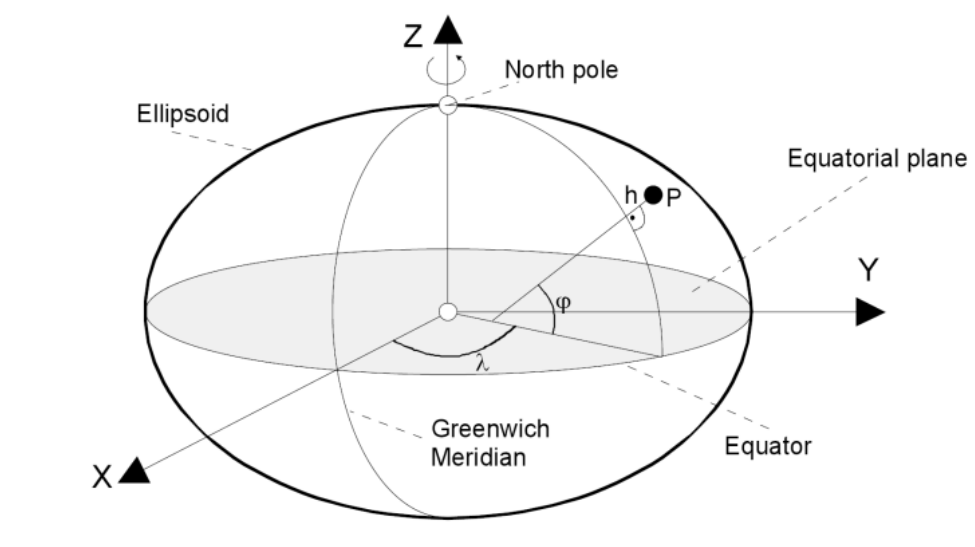
\includegraphics[width=12cm]{figures/ellipsoid}
	\caption{橢球座標系}
	\caption*{來源:MTi-G Manual}
	\label{f:ellipsoid}
\end{figure}

橢球座標系會隨著定義的橢球不同而改變,而用來描述地球所定義的橢球就稱為大地基準(Datum)。
MTi-G位置感測器使用WGS84大地基準,而這個基準也是一般GPS所使用的標準座標系,
如圖~\ref{f:ecef}所示,而參數如表~\ref{t:wgs84}所示:
\begin{table}[h!]
	\centering
	\caption{WGS84大地基準參數}
	\label{t:wgs84}
	\begin{tabular}{ | l | c | }
		\hline
		長軸$a$ & $6378137m$ \\ \hline
		短軸$b$ & $6356752.3142m$ \\ \hline
		扁率$f$	& = $(a-b) / a = 1/298.257223563$ \\
		\hline
	\end{tabular}
\end{table}

另外要注意的是,在橢球上緯度的定義有三種:
地心(Geocentric)、修化(Reduced)與測地(Geodetic)緯度~\cite{Jekeli:2006:GRSinGeodesy}。
而最常見的緯度定義,包括WGS84,都是定義為測地緯度,
其定義為:若$P$為橢球座標系上的一點,則能夠找出一過該點的經度平面(Meridian Plane),
而測地緯度$\phi$為在此平面上,過$P$點且與該橢圓垂直的直線與長軸的夾角,
如圖~\ref{f:geodetic_latitude}所示。
\begin{figure}[h!]
	\centering
	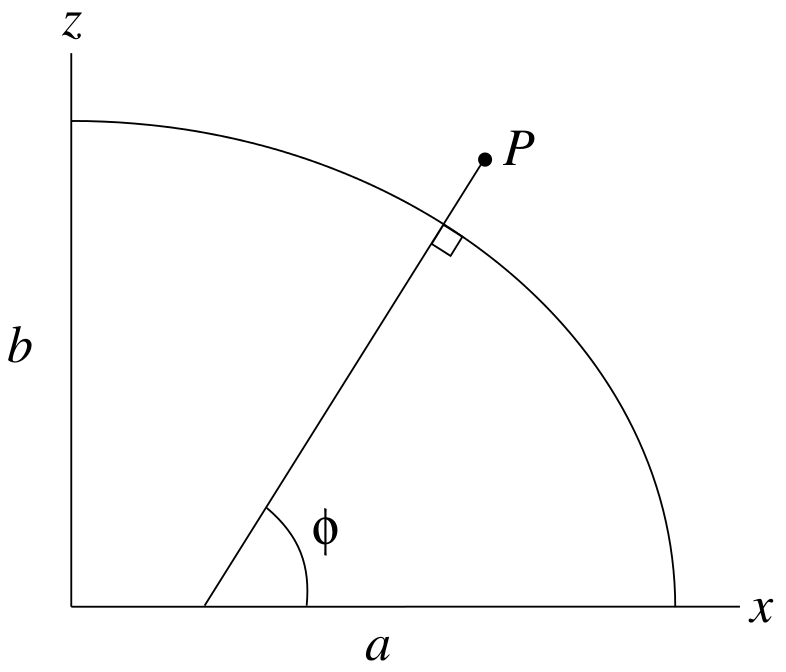
\includegraphics[width=6cm]{figures/geodetic_latitude}
	\caption{測地緯度示意圖}
	\label{f:geodetic_latitude}
\end{figure}

\subsection{測地線}
測地線(Geodesic)在微分幾何學上有嚴謹的定義,
而在橢球曲面上可視為兩點之間的最短距離~\cite{Karney:2013:Algorithms_for_Geodesics}。
與其相關的問題可分為兩種:Direct與Inverse,
前者為給定起點$A(\phi_1,\lambda_1)$、方位角(azimuth)$\alpha_1$與距離$s_{12}$後計算終點位置$B$;
後者則是給定起點$A(\phi_1,\lambda_1)$與終點$B(\phi_2,\lambda_2)$,計算兩者之間的方位角$\alpha_1$與最短距離$s_{12}$,
如圖~\ref{f:geodesic}所示~\cite{Jekeli:2006:GRSinGeodesy}。
\begin{figure}[h!]
	\centering
	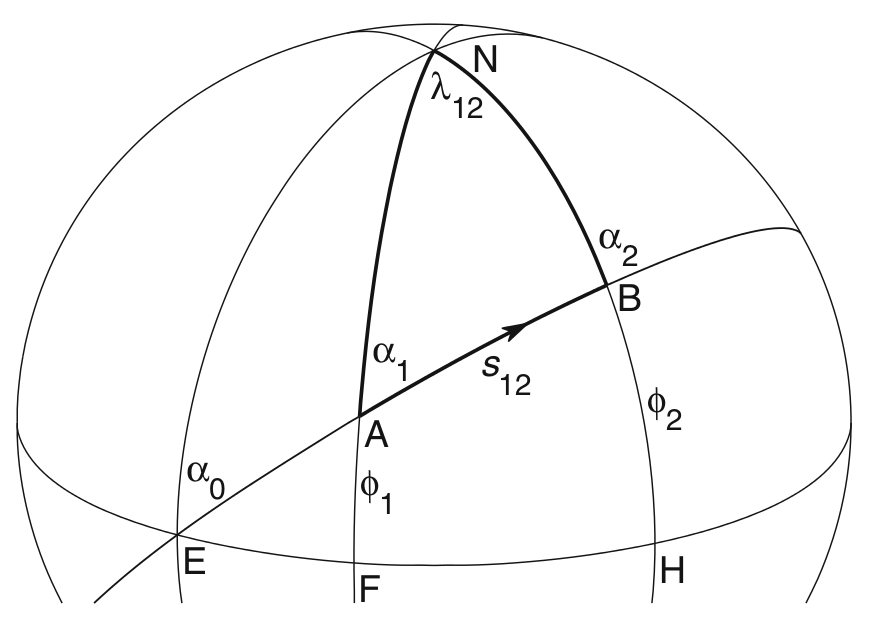
\includegraphics[width=6cm]{figures/geodesic}
	\caption{測地線}
	\label{f:geodesic}
\end{figure}

本論文需要計算兩個位置之間(車輛與目標點)的方位角與距離,因此必須要解決上述的Inverse問題。
而測地線是微分幾何學上一個重要的研究對象,當曲面較為複雜時需要非常繁瑣的計算才能得到精準值,
詳細解法可參照~\cite{Karney:2013:Algorithms_for_Geodesics,Jekeli:2006:GRSinGeodesy}。
然而,由於電腦計算能力大幅增加,已經可以使用數值方法來解決Inverse問題:
假設$\alpha_1$為已知,因此利用已知的$\phi_1$、$\phi_2$及$\alpha_1$,
可以計算出相應的$\lambda_{12} = \lambda_2 - \lambda_1$,
因此便可利用牛頓法迭代$\alpha_1$以得到正確的$\lambda_{12}$,
此時的$\alpha_1$就是正確的解,同時也可計算出相應的$s_{12}$,
也就是車輛與目標點之間的距離$\sigma_t$~\cite{Karney:2013:Algorithms_for_Geodesics}。
本論文使用GeographicLib函式庫~\cite{website:GeographicLib}處理這個問題。

\subsection{區域座標系統}
區域切平面(Local Tangent Plane)為姿態量測系統的參考座標系,
其X軸指向正北方且與橢球相切,如圖~\ref{f:LTP}所示。
其量測的姿態角即為感測器座標系統相對於此座標系統之Cardan Angle,
即航空學上常用的Roll($\phi$)、Pitch($\theta$)與Yaw($\psi$)角。
\begin{figure}[h!]
	\centering
	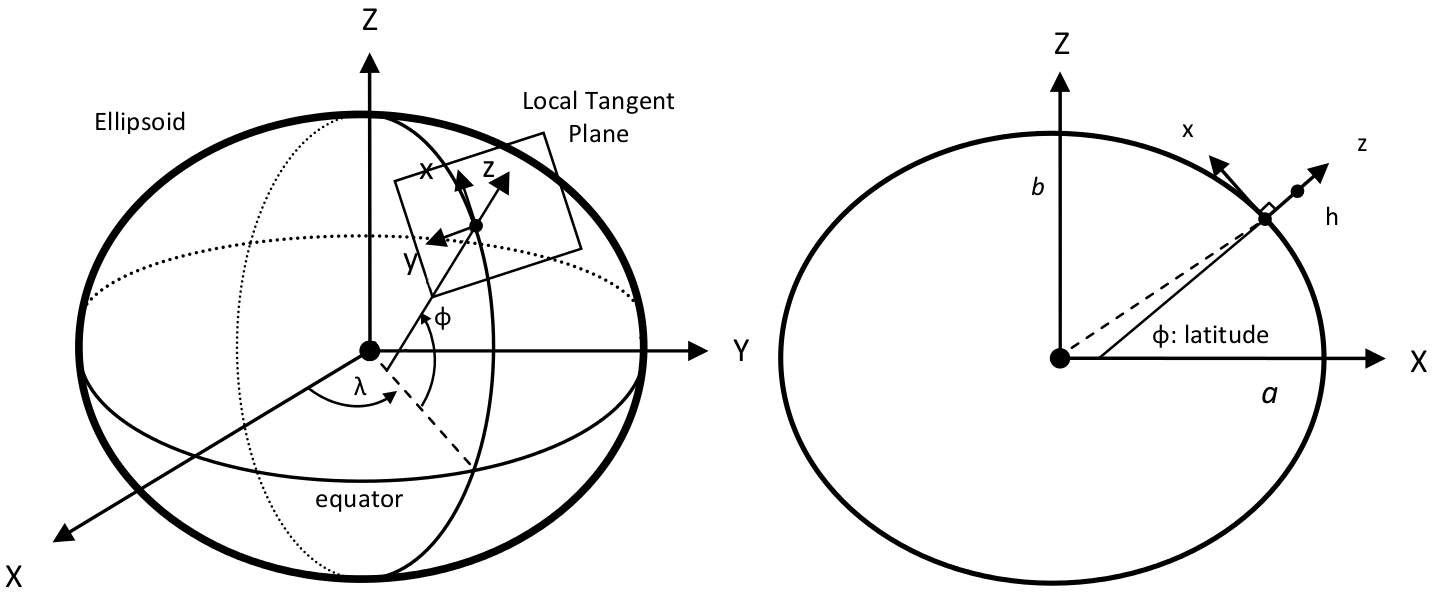
\includegraphics[width=\textwidth]{figures/LTP}
	\caption{區域切平面示意圖}
	\caption*{來源:MTi-G Manual}
	\label{f:LTP}
\end{figure}

上一節所述之方位角$\alpha_1$為相對於北方順時針方向所量測的角度;
Yaw角度$\psi$為相對於北方逆時針方向量測之角度。因此,目標方向$\Theta_t$相對於車輛之角度可依下式計算:
\begin{equation}
	\Theta_t = -\alpha_1 - \psi
\end{equation}
若$\Theta_t$為負值代表目標在車輛右側,若為正值則於位車輛左側,如圖~\ref{f:target_angle}所示。
\begin{figure}[h!]
	\centering
	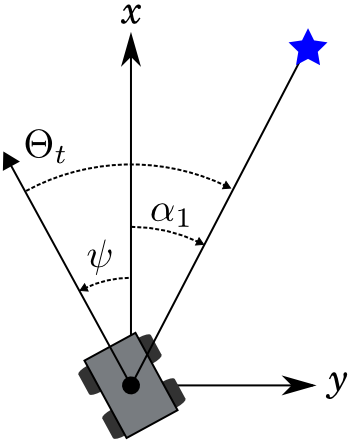
\includegraphics[width=5cm]{figures/TargetAngle}
	\caption{目標方向相對於車輛之角度}
	\label{f:target_angle}
\end{figure}

\section{避障演算法}
\label{sec:vfhplus}

\subsection{常見演算法介紹}

\subsubsection{Artificial Potential Field}
Artificial Potential Field~\cite{Khatib:1985:APF}
使用環境資訊建立一虛擬力場,讓障礙物對機器人施加排斥力,
目標點則對其施加吸引力,兩者之合力即為機器人需要前進的方向。
藉由已知的地圖或是感測器所得到的資訊,能夠計算出一位能場$U(x,y)$,
其中障礙物具有較高的位能,而目標點具有較低的位能,
如圖~\ref{f:potential_field}所示。
接著對這個位能場做梯度運算,即可得到一虛擬力場$F(x,y)$:
\begin{equation}
	F(x,y) = -\nabla U(x,y)
\end{equation}
利用此虛擬力場,便能夠計算機器人在每個位置所需要的導航方向, 
指引機器人遠離障礙物並接近目標點。
\begin{figure}[h!]
	\centering
	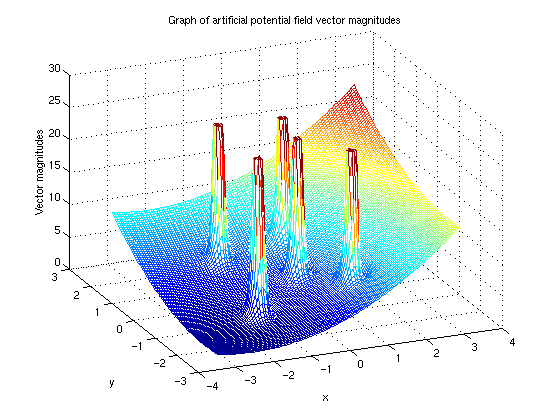
\includegraphics[width=10cm]{figures/demo_apf_whitebg}
	\caption{位能場}
	\caption*{來源:people.csail.mit.edu}
	\label{f:potential_field}
\end{figure}

此演算法不只能夠做障礙物迴避,只要有地圖資訊也同時具有全域路徑規劃的能力,而且計算效率高。
然而此演算法假設機器人為單一質點,忽略機器人的動態拘束(最大加速度、機構拘束等)及幾何尺寸,
且於狹窄的空間中表現較差。

\subsubsection{Vector Field Histogram}
Vector Field Histogram(VFH)~\cite{Borenstein:1991:VFH}
將環境資訊以極座標直方圖(Polar Histogram)$D$的方式表示,橫軸為障礙之角度$\theta$,縱軸為其距離$d$,
如圖~\ref{f:vfh}所示。接著找出可供機器人通過的空間,並計算其相對應的轉向角度。
\begin{figure}[h!]
	\centering
	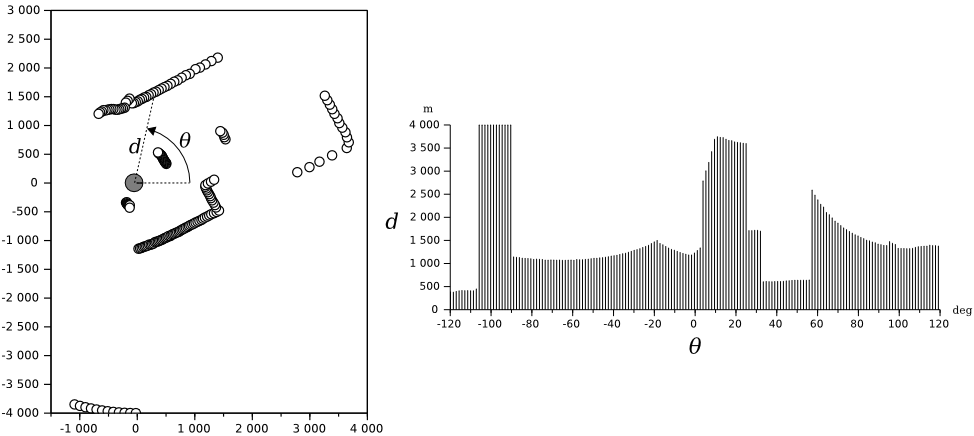
\includegraphics[width=\textwidth]{figures/VFHTotal.png}
	\caption{極座標直方圖}
	\label{f:vfh}
\end{figure}

經過此計算後可能會出現多個可通過的候選轉向角度$\alpha_n$,此時可以使用成本函數(Cost Function)$G$
來計算每個轉向角度所要花費的「成本」:
\begin{equation}
	G = \mu_1 \delta_1 + \mu_2 \delta_2 + \mu_3 \delta_3
\end{equation}
其中$\delta_1$為目標方向與$\alpha_n$的差異;$\delta_2$為目前車輛方位角與$\alpha_n$的差異;
$\delta_3$為前一次計算得到的轉向角度與$\alpha_n$的差異,
而$\mu_1$、$\mu_2$與$\mu_3$代表的是各個差異值的權重系數。
$G$所計算出的值代表選擇該$\alpha_n$所需要耗費的成本,
藉由調整權重系數也能改變機器人導航時的趨勢。

VFH的極座標直方圖可直接套用光學雷達所得到的資訊,計算速度也相當快,
而且藉由成本函數也能夠調整機器人的導航特性。然而VFH並沒有考慮機器人的動態拘束與幾何尺寸,
而且\textbf{VFH所計算的轉向角度是由可通過的空間所決定的,並非目標方向}。
這是一個相當重要的特性,在狹窄的室內空間中這不會造成太大的影響,
然而在較為寬廣、障礙物較少的室外空間中,若光學雷達沒有偵測到障礙物,
此時演算法只會找到一個可通過的空間,以圖~\ref{f:vfh}來說就是從$-120\,^{\circ}$到$120\,^{\circ}$的範圍,
所以機器人只會朝著唯一的方向─正前方前進,直到偵測到障礙物,因此VFH並不適用於本論文。

\subsubsection{Curvature Velocity Method}
Curvature Velocity Method(CVM)~\cite{Simmons:1996:CVM}
考慮機器人的動態拘束,假設機器人的運動軌跡為曲率$c=\omega/\nu$的圓弧,
其中$\omega$代表機器人的旋轉速度(Rotational Velocity),$\nu$則是直線速度(Translational Velocity),
如圖~\ref{f:cvm_curvature}所示。因此,CVM使用速度空間$(\nu,\omega)$來做路徑規劃,而非卡式座標空間。
\begin{figure}
	\centering
	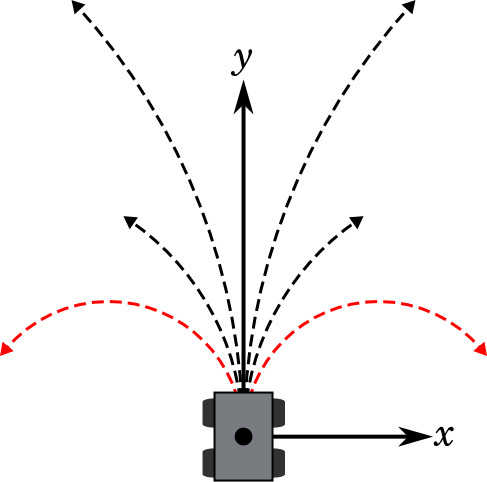
\includegraphics[width=8cm]{figures/CVM1}
	\caption{CVM下的機器人運動軌跡}
	\label{f:cvm_curvature}
\end{figure}

為了將障礙物轉換至速度空間,設定一距離函數$D(c,OBS)$為沿著曲率$c$行走直到與障礙物集合$OBS$接觸的距離。
接著設定一最大行走距離$L$,表示機器人所能感測到的最大距離,此時距離函數將成為$D_{limit}$:
\begin{equation}
	D_{limit}(c,OBS) = min(L,D(c,OBS))
\end{equation}
為了計算方便,CVM將障礙物簡化為圓形,因此便能快速的將障礙物資訊轉換至速度空間。

CVM同樣使用一目標函數(Objective Function)$f$計算最佳的$\nu$與$\omega$:
\begin{equation}
	f(\nu,\omega) = \mu_1 \cdot speed(\nu) + \mu_2 \cdot dist(\nu,\omega) + \mu_3 \cdot head(\omega)
\end{equation}
其中:
\begin{align*}
	speed(\nu)	&= \nu / \nu_{max} \\ 
	dist(\nu,\omega)	&= D_{limit}({\omega \over \nu},OBS) / L \\
	head(\omega)	&= 1 - |\theta_{target} - \omega \cdot T_{c} | / \pi \\
\end{align*}
$\nu_{max}$為最大直線速度,$\theta_{target}$為目標方向,$T_c$為一時間常數。
此函數與先前的成本函數相反,產生最大值的$(\nu,\omega)$才是最佳值。

CVM藉由速度空間設定動態拘束,可設定最大速度與最大加速度來限制其運動狀態。
幾何拘束也可利用放大障礙物的尺寸來調整。然而過於簡化的障礙物是其限制,
而且必須具備速度感測器才能使用此演算法,因此不適用於本論文。

\subsubsection{Dynamic Window Approach}
Dynamic Window Approach(DW)~\cite{Thrun:1997:DW}
與CVM相同,假設機器人之運動軌跡為曲率$c=\omega/\nu$的圓弧,
利用最大直線速度與最大旋轉速度建立一速度空間,並將量測到的環境轉換至此空間中,
如圖~\ref{f:DW_cartesian}及~\ref{f:DW_velocity}所示。
\begin{figure}[h!]
	\centering
	\begin{subfigure}[t]{0.6\textwidth}
		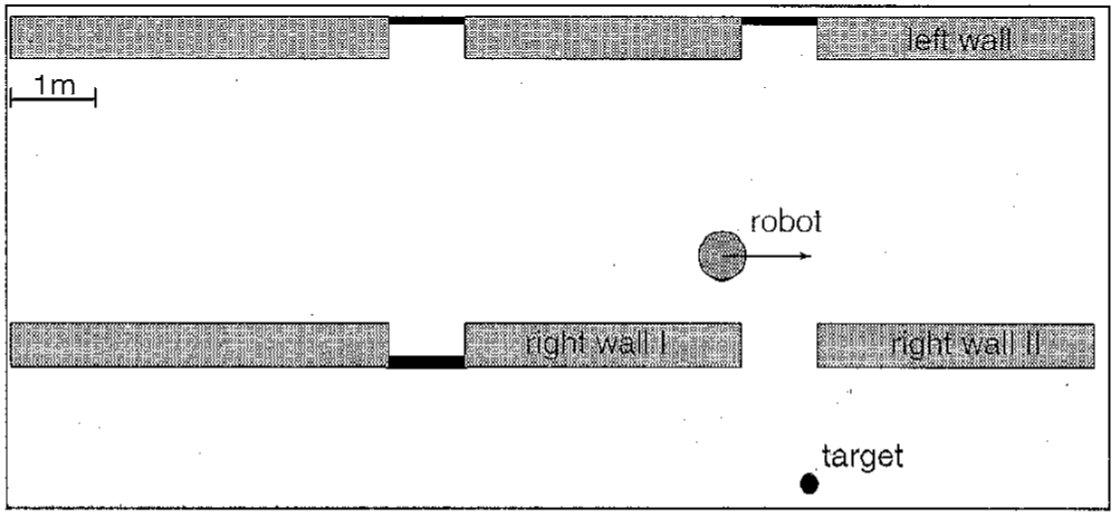
\includegraphics[width=\textwidth]{figures/DW_cartesian}
		\caption{實際環境資訊}
		\label{f:DW_cartesian}
	\end{subfigure}
	\begin{subfigure}[t]{0.6\textwidth}
		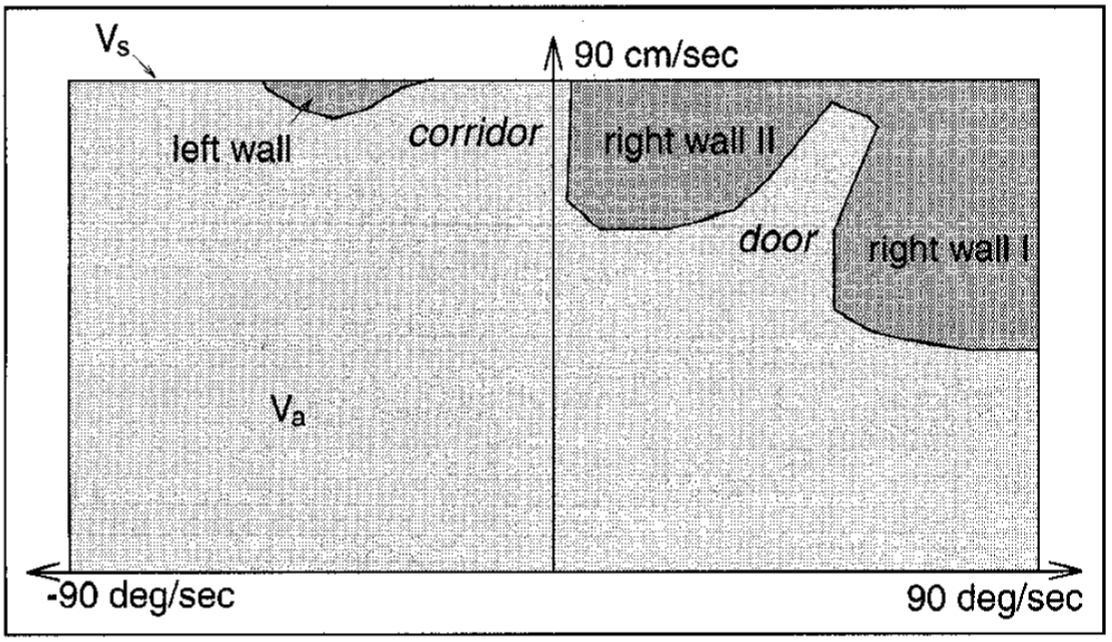
\includegraphics[width=\textwidth]{figures/DW_velocity}
		\caption{速度空間中的環境資訊}
		\label{f:DW_velocity}
	\end{subfigure}
	\caption{環境資訊轉換}
	\caption*{來源:The Dynamic Window Approach to Collision Avoidance}
	\label{f:v_space}
\end{figure}
在圖~\ref{f:DW_velocity}中橫軸為旋轉速度,縱軸為直線速度;較暗的部分為被障礙物擋住的部分。

在速度空間中,根據機器人目前的速度以及最大加速度,可在速度空間中找出一動態視窗(Dynamic Window)$V_d$,
此視窗根據最大加速度限制了機器人所能達到的速度(視窗大小),
隨著機器人目前的速度不同此視窗的位置也會不斷改變,如圖~\ref{f:dynamic_window}所示。
\begin{figure}[h!]
	\centering
	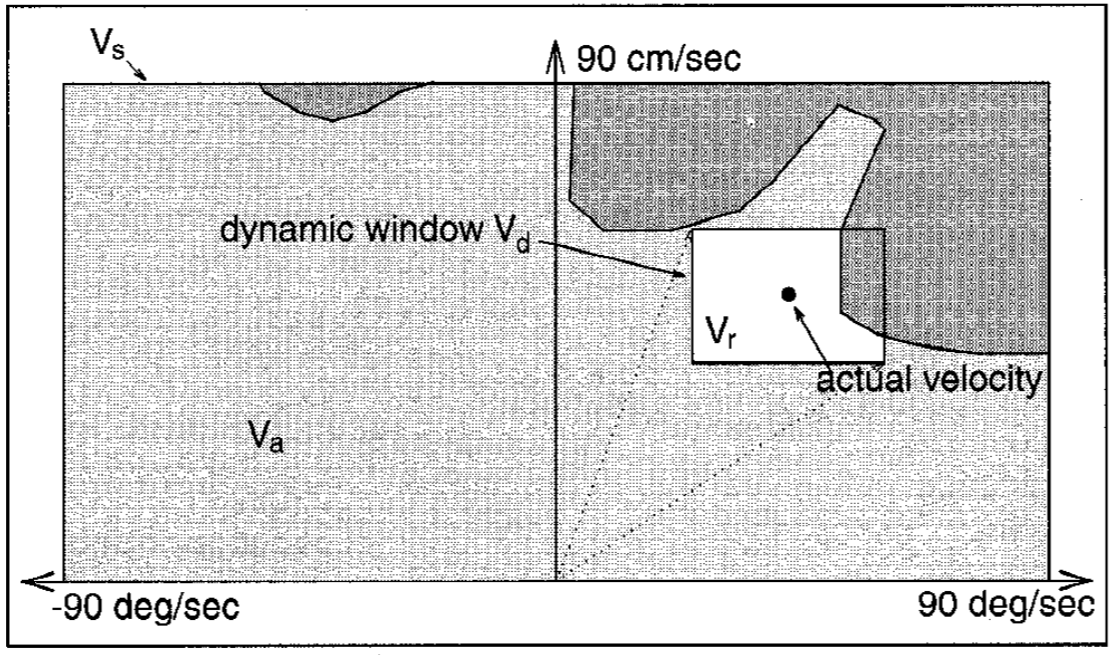
\includegraphics[width=10cm]{figures/dynamic_window}
	\caption{動態視窗示意圖}
	\caption*{來源:The Dynamic Window Approach to Collision Avoidance}
	\label{f:dynamic_window}
\end{figure}
此視窗中的所有速度$(\nu,\omega)$代表了機器人所有可能達到的速度,而為了在此視窗中找出最佳解,
DW同樣使用目標函數來做最佳化。

藉由改變速度空間的形狀,DW能夠設定機器人的機構運動拘束,而動態視窗則考慮了機器人的動態拘束。
然而DW的計算較為複雜,且與CVM相同,都必須裝設速度感測器才能使用此演算法,因此並不適用於本論文。

\subsection{Vector Field Histogram Plus}
Vector Field Histogram Plus(VFH+)~\cite{Ulrich:1998:VFHPlus}
改進了許多VFH的缺點,將機器人的幾何限制和運動拘束也考慮在內。

原先的VFH+使用四個階段的計算逐一減少資訊量並找出轉向角度,而為了使用在光學雷達上,
本論文一樣使用四個階段的計算,但修改其計算方式與順序以便使用於光學雷達。
前面三個階段著重於根據機器人的拘束找出可通過的方向,最後一個階段則是計算最佳方向。
另外,除了計算避障的轉向外,VFH+也可根據環境資訊控制機器人之速度,

\subsubsection{階段一、極座標直方圖}
光學雷達所量測到的資訊可表示為$d_i$與$\theta_i$,$d_i$為第$i$個量測到的距離,
$\theta_i$則為$d_i$所對應的角度,如圖~\ref{f:LiDar_measurement}所示。
\begin{figure}[h!]
	\centering
	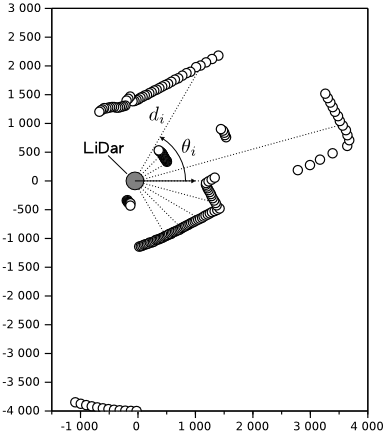
\includegraphics[width=8cm]{figures/LiDar_measurement}
	\caption{光學雷達量測示意圖}
	\label{f:LiDar_measurement}
\end{figure}

與VFH相同,VFH+首先使用光學雷達所得到的資訊建立一極座標直方圖$P_i$:
\begin{equation}
	P_i = a - b\cdot d_i
\end{equation}
$a$與$b$皆為正值。藉由調整此處的$a$與$b$,使用者可調整VFH+所要偵測與計算的範圍。
圖~\ref{f:polar_histogram}為$a=1200$、$b=1$的設定下,
圖~\ref{f:LiDar_measurement}所量測到之環境產生的$d_i$與$P_i$示意圖。
\begin{figure}[h!]
	\centering
	\begin{subfigure}[b]{0.7\textwidth}
		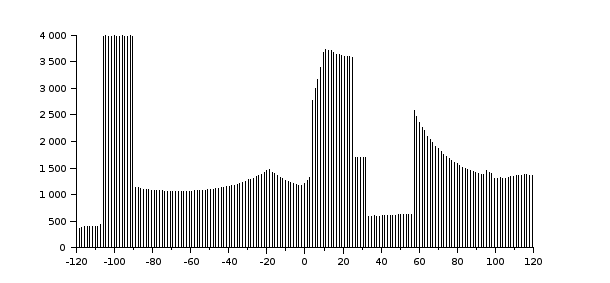
\includegraphics[width=\textwidth]{figures/polar_histogram}
		\caption{$d_i$}
		\label{f:polar_histogram_original}
	\end{subfigure}
	\begin{subfigure}[b]{0.7\textwidth}
		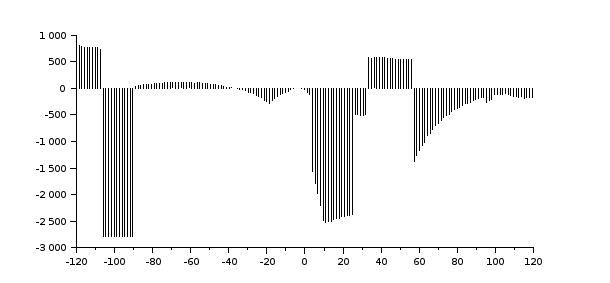
\includegraphics[width=\textwidth]{figures/polar_histogram_modified}
		\caption{$P_i$}
		\label{f:polar_histogram_modified}
	\end{subfigure}
	\caption{極座標直方圖}
	\label{f:polar_histogram}
\end{figure}

\subsubsection{階段二、安全空間}
為了找出可供機器人通過的空間,VFH藉由一閾值$\tau$過濾出所有視為安全的距離,
而一段連續的安全距離就代表一個可通過的安全空間$V_j$,由一組邊界向量$(\mathbf{B_l},\mathbf{B_r})_j$定義,
定義其左邊界與右邊界的角度$\theta$與障礙物的距離$d$,視為機器人所能通過的方向:
\begin{align}
	\mathbf{B_l}	&= \begin{bmatrix}
				\theta_l & d_l
			   \end{bmatrix} \nonumber \\
	\mathbf{B_r}	&= \begin{bmatrix}
				\theta_r & d_r
			   \end{bmatrix}
	\label{e:boundary}
\end{align}
然而VFH只使用單一閾值可能會過濾出許多不連續的空間,
造成許多不必要的方向選擇出現,讓機器人在決定方向時產生左右搖擺的現象。
因此,VFH+使用兩個閾值$\tau_{max}$與$\tau_{min}$,
利用遲滯(Hysteresis)效果過濾掉這些不必要的空間,產生二元直方圖(Binary Histogram)$H_i$:
\begin{equation}
	H_i = 
	\begin{cases}
		1	& \textrm{if } P_i \geq \tau_{max} \\
		0	& \textrm{if } P_i \leq \tau_{min} \\
		H_{i-1}	& \textrm{otherwise}
	\end{cases}
\end{equation}
圖~\ref{f:binary_histogram_1}為使用單一門檻值$\tau=0$的過濾結果,圖~\ref{f:binary_histogram_2}
則為使用雙閾值$\tau_{min}=0,\tau_{max}=450$的過濾結果,值為$0$的區域代表可通過的安全空間。
圖中可看到單閾值過濾產生了四個區域,而雙閾值則只有二個。
\begin{figure}[h!]
	\centering
	\begin{subfigure}[b]{0.8\textwidth}
		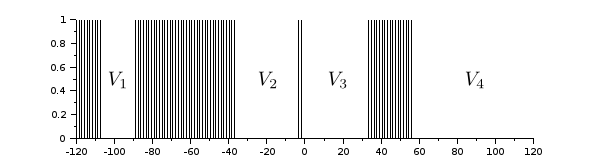
\includegraphics[width=\textwidth]{figures/binary_histogram_1}
		\caption{單一閾值}
		\label{f:binary_histogram_1}
	\end{subfigure}
	\begin{subfigure}[b]{0.8\textwidth}
		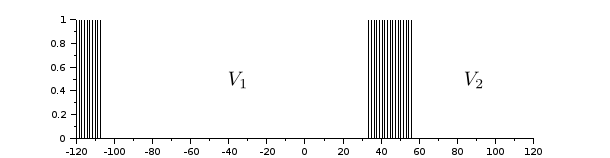
\includegraphics[width=\textwidth]{figures/binary_histogram_2}
		\caption{雙閾值}
		\label{f:binary_histogram_2}
	\end{subfigure}
	\caption{過濾結果比較}
	\label{f:binary_histogram}
\end{figure}

原先的VFH忽略了機器人本身的幾何尺寸,而本論文使用縮小安全空間$V_j$邊界的方式來增加幾何拘束,
此時便可將機器人視為一質點。假設機器人之尺寸為半徑$w_s$的圓,則將$V_j$之邊界同樣縮小$w_s$後
便可將機器人視為一點,如圖~\ref{f:width}所示。
縮減後的安全空間$\hat{V_j} = (\hat{\mathbf{B_l}},\hat{\mathbf{B_r}})_j$可由式~\ref{e:width}計算:
\begin{align}
	\hat{\mathbf{B_l}}	&= \begin{bmatrix}
					\theta_l - \delta_l & d_l\cos\delta_l
				   \end{bmatrix},\delta_l = \arcsin({\frac{w_s}{d_l}}) \nonumber \\
	\hat{\mathbf{B_r}}	&= \begin{bmatrix}
					\theta_r + \delta_r & d_r\cos\delta_r
				   \end{bmatrix},\delta_r = \arcsin({\frac{w_s}{d_r}})
	\label{e:width}
\end{align}

在計算邊界縮減時,有時會發生邊界交疊$\theta_r + \delta_r > \theta_l - \delta_l$的情況,
這代表此安全空間無法讓機器人通過,此時該安全空間會被捨棄,如圖~\ref{f:width_overlapped}所示。
\begin{figure}[h!]
	\centering
	\begin{subfigure}[t]{0.5\textwidth}
		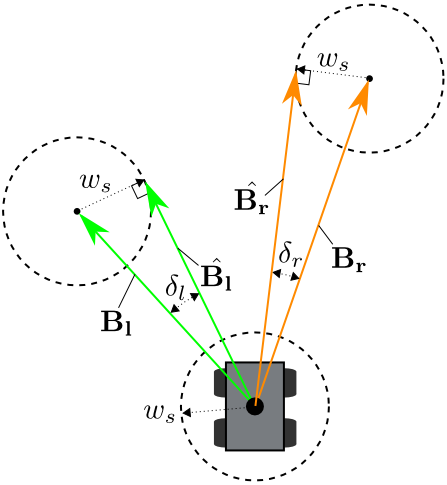
\includegraphics[width=\textwidth]{figures/width}
		\caption{邊界縮減}
		\label{f:width}
	\end{subfigure}
	~
	\begin{subfigure}[t]{0.32\textwidth}
		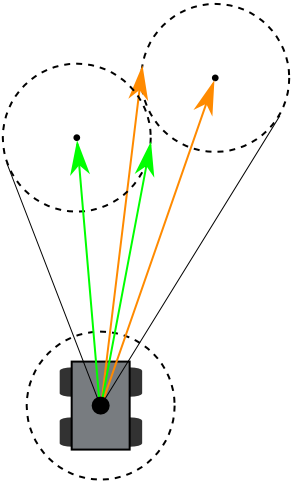
\includegraphics[width=\textwidth]{figures/width_overlapped}
		\caption{邊界交疊}
		\label{f:width_overlapped}
	\end{subfigure}
	\caption{邊界處理}
\end{figure}

\subsubsection{階段三、Blocked Directions}
VFH並沒有將機器人的動態拘束納入考慮,其假設所有轉向角度都是可達成的,然而這對某些轉向機構來說是不可能的。
因此VFH+使用機器人的最小迴轉半徑$R$與機器人尺寸$w_s$,計算出被障礙物所限制住的轉向角度$(\phi_l,\phi_r)$。
而原先的VFH+僅使用迴轉半徑$R$來計算,而本論文將機器人尺寸$w_s$加入計算,形成與迴轉半徑同心但半徑為$R+w_s$的圓,
如圖~\ref{f:block_directions}所示。
\begin{figure}
	\centering
	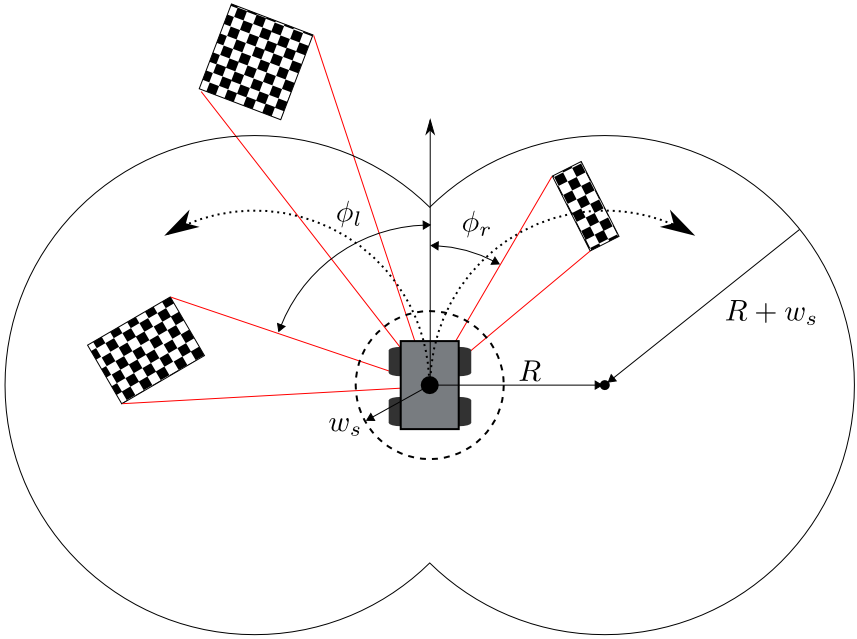
\includegraphics[width=0.8\textwidth]{figures/block_directions}
	\caption{轉向角度限制}
	\label{f:block_directions}
\end{figure}

為了找出$(\phi_l,\phi_r)$,首先使用與光學雷達相同的$\theta_i$建立一偵測距離用的直方圖$D_i$,
如圖~\ref{f:detection_histogram}所示,其可由式~\ref{e:detection_histogram}計算。
\begin{figure}[h!]
	\centering
	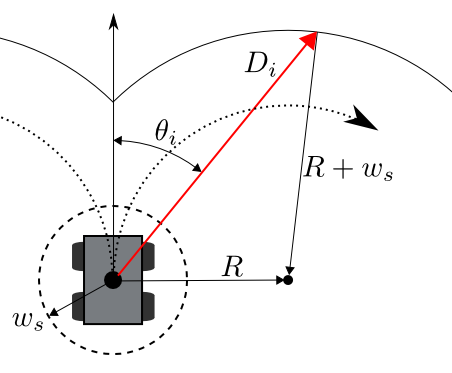
\includegraphics[width=0.5\textwidth]{figures/detection_histogram}
	\caption{偵測直方圖示意圖}
	\label{f:detection_histogram}
\end{figure}
\begin{equation}
	D_i = |R\sin\theta_i| + \sqrt{R^2\sin^2\theta_i + w_s^2 + 2Rw_s}
	\label{e:detection_histogram}
\end{equation}
接著將光學雷達測得的$d_i$與$D_i$相減,所得到的直方圖稱為$M_i$
\begin{equation}
	M_i = d_i - D_i
\end{equation}
若$M_i$中對應於$\theta_i$之值小於$0$,則代表$\theta_i$有障礙物位於機器人之最小迴轉範圍內,
必須改變$(\phi_l,\phi_r)$限制轉向角度以避開障礙物。
環境與這些直方圖之間的轉換如圖~\ref{f:histogram_transform}所示。
\begin{figure}[h!]
	\centering
	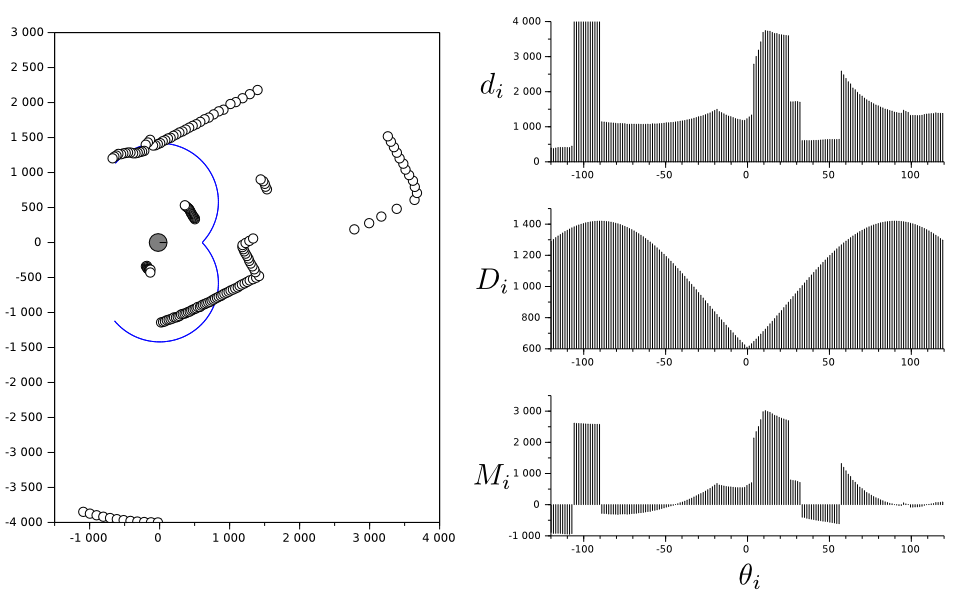
\includegraphics[width=\textwidth]{figures/histogram_transform}
	\caption{直方圖轉換}
	\label{f:histogram_transform}
\end{figure}

利用$M_i$,$(\phi_l,\phi_r)$可以非常快速的被計算出來:
\begin{enumerate}
	\item{首先設$\phi_l = \pi$、$\phi_r = -\pi$}
	\item{對所有$i$,若$M_i < 0$:}
		\begin{enumerate}
			\item{若$\theta_i < 0$且$\theta_i > \phi_r$,則將$\phi_r$設為$\theta_i$}
			\item{若$\theta_i > 0$且$\theta_i < \phi_l$,則將$\phi_l$設為$\theta_i$}
		\end{enumerate}
\end{enumerate}

\subsubsection{階段四、Selection of Steering Direction}
根據安全空間$V_j$的寬度,可以從每個$V_j$中找到一個或多個候選方向$c$,
接著使用成本函數於這些候選方向中找出最佳解。
對於安全空間的寬度,本論文使用其邊界向量之間的角度差$\epsilon = \theta_l - \theta_r$做為判斷標準,
使用一角度閾值$\tau_a$將安全空間分為兩種:狹窄與寬廣。

對狹窄($\epsilon < \tau_a$)的安全空間來說,只有正中央的方向是唯一的候選方向:
\begin{equation}
	c_n = \frac{\theta_l + \theta_r}{2}
\end{equation}

而對寬廣($\epsilon > \tau_a$)的安全空間來說則有兩個,分為兩邊界向量所對應的角度。
另外若目標方向$\Theta_t$位於該安全空間中,則目標方向也會是候選角度的其中之一:
\begin{align}
	c_r &= \theta_r \nonumber \\
	c_l &= \theta_l \nonumber \\
	c_t &= \Theta_t 
\end{align}

最後使用一成本函數$G$於這些候選轉向角中找出最佳解:
\begin{equation}
	G(c) = \mu_1\cdot(|c - \Theta_t|) + \mu_2\cdot(|c|) + \mu_3\cdot(|c - c_{t-1}|)
	\label{e:cost_function}
\end{equation}
在式~\ref{e:cost_function}中,第一項$(|c - \Theta_t|)$代表候選方向與目標方向之間的差距。
差距越大表示該候選角會將機器人帶離目標方向,所以成本將會增加。

第二項$(|c|)$代表候選方向與目前車輛方向的差距。這些候選角都是以車身座標系做為參考,
所以車輛本身方位角相對於此座標系將永遠是$0$,而候選方向越大代表機器人將會偏離目前的方向越多,
進而增加成本。

第三項$(|c - c_{t-1}|)$則代表候選角與前一次選擇的轉向角之間的差距。
這個差距越大代表機器人的越容易偏離目前的航向,造成擺盪的現象。

$\mu_1,\mu_2,\mu_3$則是相對應的權重系數,藉由調整這三個系數之間的相對大小,
機器人的導航特性就能夠被調整,而於成本函數中產生最小值的候選方向即為最佳方向$c_t$。

\subsubsection{速度控制}
機器人的速度是藉由環境的障礙物密度來控制,若密度越高則機器人速度就必須越慢,反之則越快。
障礙物密度可藉由一密度函數$D$與一距離閾值$\tau_{obj}$計算:
\begin{equation}
	D(d_i) = \frac{1}{N}\sum_{i=1}^{N}H_i
\end{equation}
其中
\begin{equation}
	H_i = 
	\begin{cases}
		0	& \textrm{if } d_i \geq \tau_{obj} \\
		1	& \textrm{if } d_i < \tau_{obj} \\
	\end{cases}
\end{equation}

得到環境密度$D(d_i)$後,可設定一最大速度值$v_{max}$與最小速度值$v_{min}$,則速度$v$可由下式計算:
\begin{equation}
	v = (v_{max}-v_{min}) \cdot (1-D(d_i)) + v_{min}
\end{equation}

